\hypertarget{Unit4_8cpp}{
\section{/PIWO/Program/Unit4.cpp File Reference}
\label{Unit4_8cpp}\index{/PIWO/Program/Unit4.cpp@{/PIWO/Program/Unit4.cpp}}
}
{\tt \#include $<$vcl.h$>$}\par
{\tt \#include \char`\"{}Unit4.h\char`\"{}}\par


Include dependency graph for Unit4.cpp:\nopagebreak
\begin{figure}[H]
\begin{center}
\leavevmode
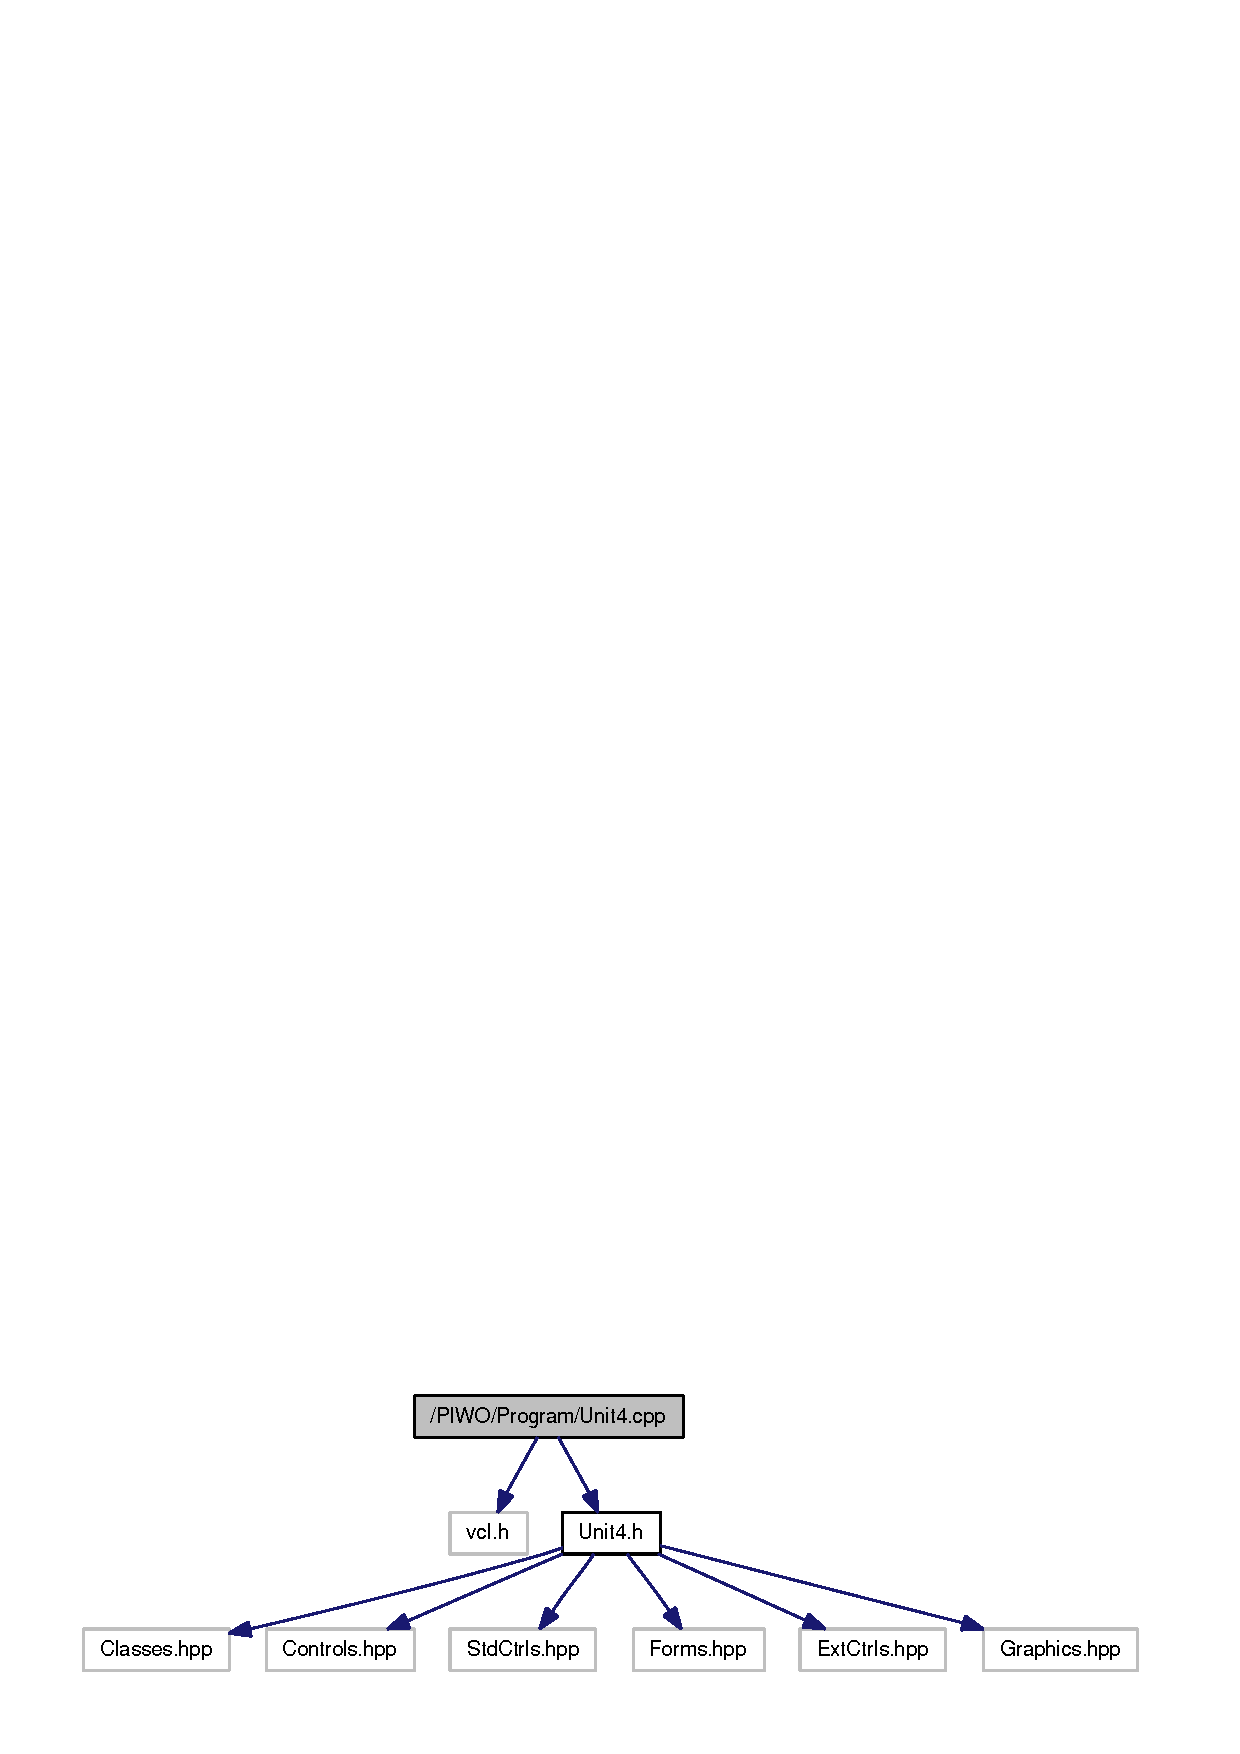
\includegraphics[width=275pt]{Unit4_8cpp__incl}
\end{center}
\end{figure}
\subsection*{Variables}
\begin{CompactItemize}
\item 
\hyperlink{classTForm4}{TForm4} $\ast$ \hyperlink{Unit4_8cpp_cea6bff5ccabaca1a21281507906feb5}{Form4}
\end{CompactItemize}


\subsection{Variable Documentation}
\hypertarget{Unit4_8cpp_cea6bff5ccabaca1a21281507906feb5}{
\index{Unit4.cpp@{Unit4.cpp}!Form4@{Form4}}
\index{Form4@{Form4}!Unit4.cpp@{Unit4.cpp}}
\subsubsection[Form4]{\setlength{\rightskip}{0pt plus 5cm}{\bf TForm4}$\ast$ {\bf Form4}}}
\label{Unit4_8cpp_cea6bff5ccabaca1a21281507906feb5}




Definition at line 11 of file Unit4.cpp.

Referenced by TForm1::Oprogramie1Click().